%
\documentclass{beamer}
\usepackage{caption}
\usepackage{subcaption}
\usepackage{pdfpages}
\usepackage{graphicx}
\usepackage{../../arbenson-math}
\usepackage[parfill]{parskip}

\usetheme{boxes}
\usecolortheme{seahorse}

\AtBeginSection[]
{
  \begin{frame}<beamer>
    \frametitle{\thesection}
    \tableofcontents[currentsection]
  \end{frame}
}

\title{CME 193: Introduction to Scientific Python \\
Lecture 7: MapReduce}
\author{
Dan Frank \\
\vspace{0.1in}
Institute for Computational and Mathematical Engineering (ICME)}
\date{January 30, 2014}
\begin{document}




\maketitle

\begin{frame}
\frametitle{Administrivia}
\begin{itemize} 
\setlength{\itemsep}{0.1in}
\item{Final HW 5 due on Feb 4 }
\item{No class Feb 2}
\end{itemize}
\end{frame}




\section{MapReduce} 

\begin{frame}
\frametitle{What is MapReduce}

\textbf{Me:} A programming paradigm that fits many computational tasks and an infrastructure to execute code written in that framework. Enables massively parallel and fault tolerant code execution over arbitrarily large datasets. The most common implementation of such an infrastructure is open-source and called Hadoop.

\textbf{Wikipedia:} MapReduce is a programming model for processing large data sets with a parallel, distributed algorithm on a cluster.

\end{frame}

\begin{frame}
\frametitle{What is MapReduce: classic map()}
A map operation takes several pieces of data and computes with each. 
No need to have this data or computation on only one machine. 
\codeblock{code/map.py}
\end{frame}

\begin{frame}
\frametitle{What is MapReduce: classic reduce()}
A reduce operation takes several pieces of data and combines them. 
Need to have all the data and computation done on one machine.
\codeblock{code/reduce.py}
\end{frame}

\begin{frame}
\frametitle{MapReduce: 3 steps}
Computation structured with \texttt{(key, value)} pairs
\begin{enumerate}
\item \texttt{mapper(key, value)} take one \texttt{(key, value)} pair as in put and output 0 or more \texttt{(key, value)} pairs
\item \texttt{shuffle/sort/groupby}: Group all of the values corresponding to the same key together (to be sent to a reducer). Taken care of for you by MapReduce infrastructure.  
\item \texttt{reducer(key, values)} take a key and a list of values as input and output 0 or more \texttt{(key, value)} pairs
\end{enumerate}
\end{frame}

\begin{frame}
\frametitle{MapReduce: 3 steps}
\begin{figure}[h]
\centering
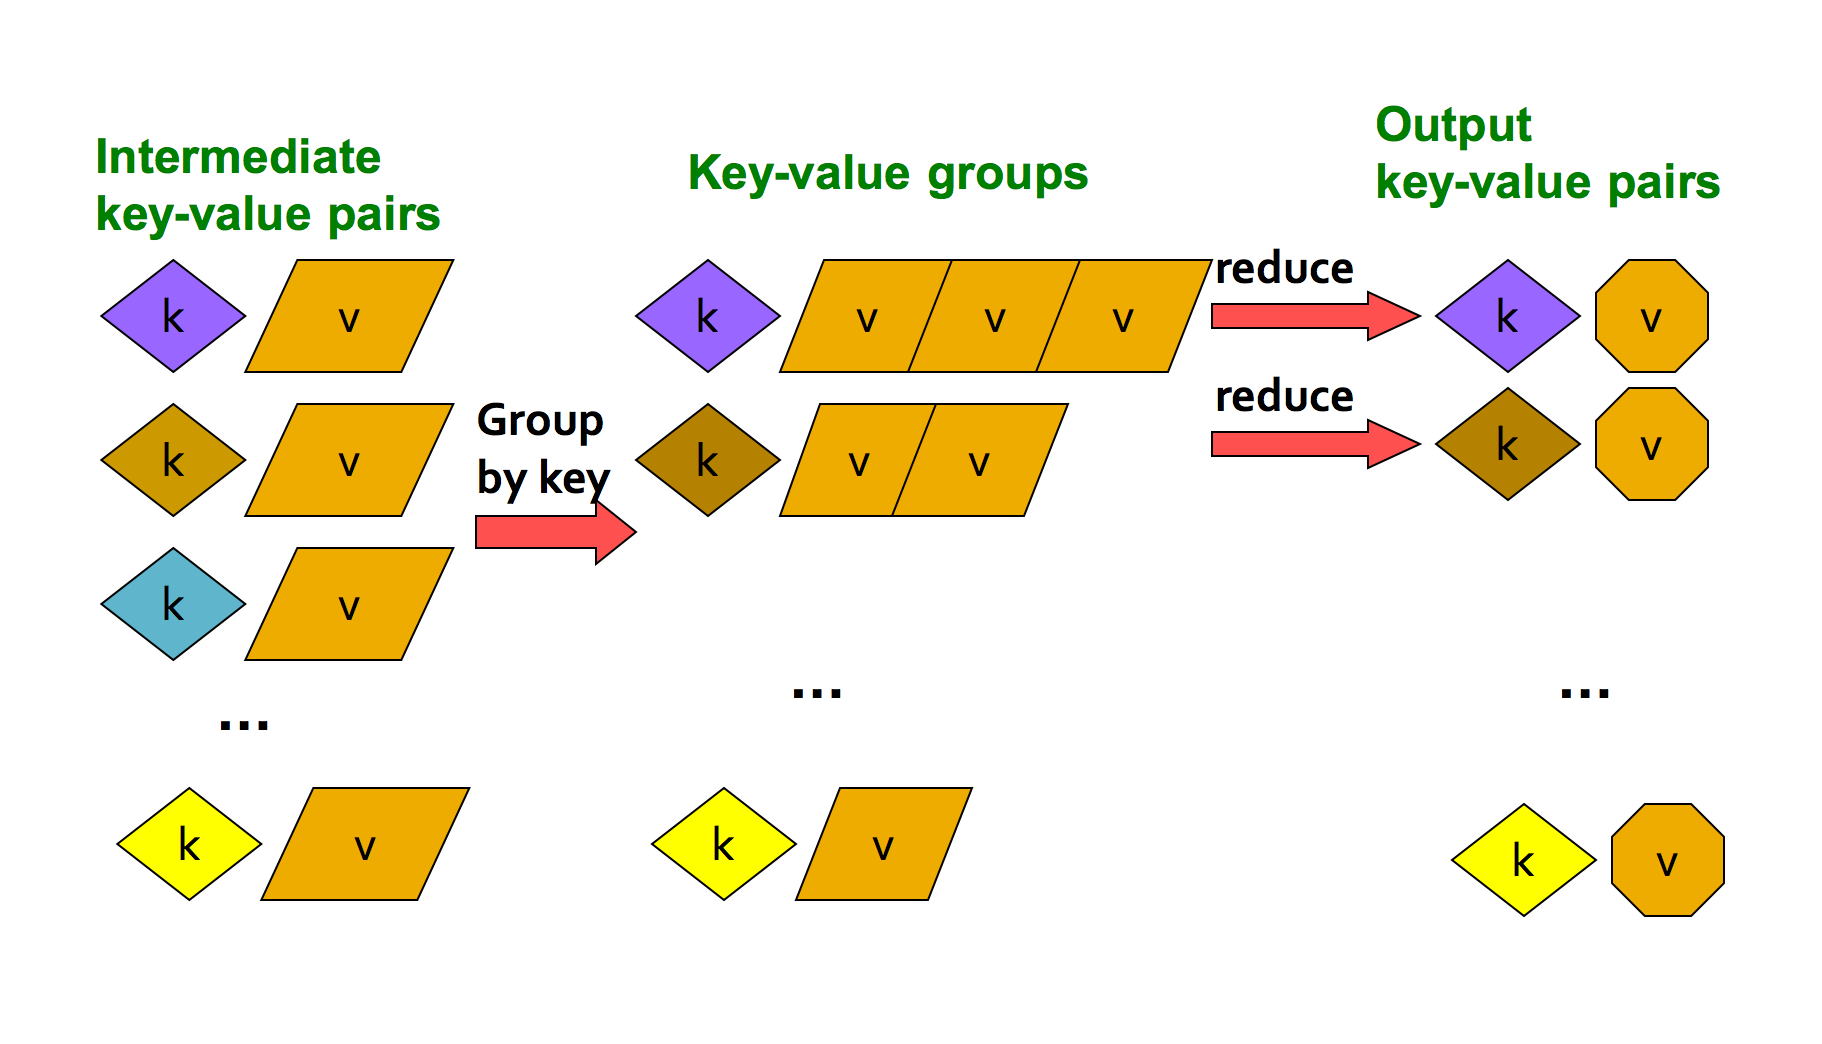
\includegraphics[width=.95\textwidth]{images/mapreduce.png}
\end{figure}
shamelessly stolen from CS246
\end{frame}




\begin{frame}
\frametitle{Aside: Python Generators \& Lazy Evaluation}
Suppose I want to represent the entire set of natural numbers in a python program. This set is infinite so we clearly can't store it in memory. But so long as we don't need to access every integer at once, we can still represent them using generators 
\codeblock{code/integer_generator.py}
\end{frame}

\begin{frame}
\frametitle{Generator Example}
\codeblock{code/generator_example.py}
\end{frame}

\begin{frame}
\frametitle{Classic example: Word Count}
Take a large file and output the counts of each word in that file. 

We'll input each line of the file into our mappers as values, ignoring the key. From each mapper we'll emit pairs consisting of (word, 1). 

The reducer will take keys and get a list of 1's as values which we will sum to get each word count.
\end{frame}

\begin{frame}
\frametitle{Classic example: Word Count}
\begin{figure}[h]
\centering
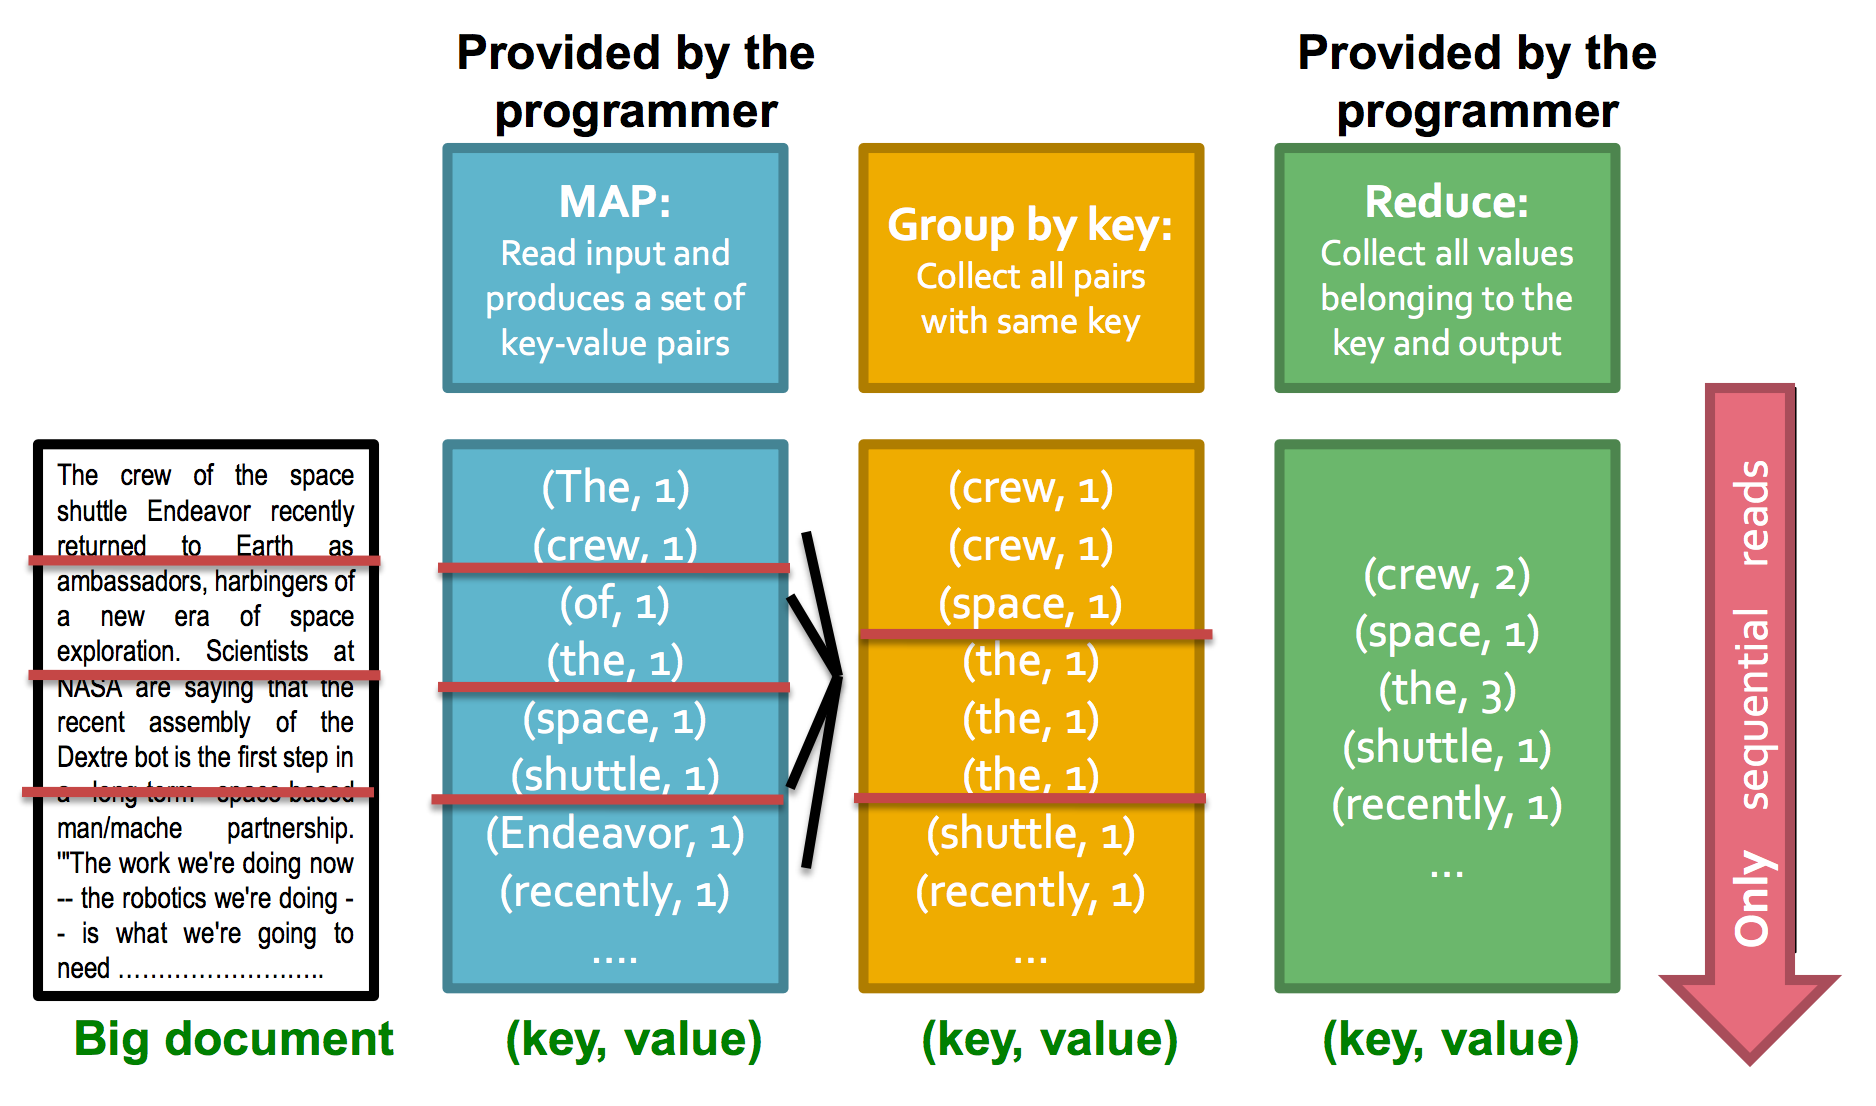
\includegraphics[width=.95\textwidth]{images/wordcount.png}
\end{figure}
shamelessly stolen from CS246
\end{frame}

\begin{frame}
\frametitle{Mapper for WordCount}
Take in one \texttt{(\_, line\_of\_text)} pair and output \text{(word, 1)} pairs
\codeblock{code/mapper.py}
\end{frame}

\begin{frame}
\frametitle{Reducer for WordCount}
Take in one \texttt{(word, list\_of\_ones)} pair and output  \text{(word, sum)} pair
\codeblock{code/reducer.py}
\end{frame}





\section{Hadoop}

\begin{frame}
\frametitle{What is Hadoop}

The standard open-source MapReduce infrastructure including...
\begin{enumerate}
\item job scheduler to execute map and reduce tasks with appropriate data 
\item job tracking to re-execute failed jobs
\item storage infrastructure: distributed file system (HDFS)
\end{enumerate}
\end{frame}

\begin{frame}
\frametitle{Hadoop Setup}

How do we hook up our code to a MapReduce infrastructure... especially since it's written in Java.
\begin{enumerate}
\item\textcolor{blue}{\href{http://www.michael-noll.com/tutorials/running-hadoop-on-ubuntu-linux-single-node-cluster/}{Running Hadoop On Ubuntu Linux (Single-Node Cluster)}} - How to set up a pseudo-distributed, single-node Hadoop cluster backed by the Hadoop Distributed File System (HDFS)
\item \textcolor{blue}{\href{http://www.michael-noll.com/tutorials/running-hadoop-on-ubuntu-linux-multi-node-cluster/}{Running Hadoop On Ubuntu Linux (Multi-Node Cluster)}} -  How to set up a distributed, multi-node Hadoop cluster backed by the Hadoop Distributed File System (HDFS)
\end{enumerate}
\end{frame}



\begin{frame}
\frametitle{Hadoop Streaming}
Mostly Hadoop expects us to be writing in Java or at least Jython, but we'd like to keep writing pure python, so we can instead use Hadoop Streaming which passes key values to an executable. In our case this will be python.

The values are passed via standard input and output values are expected to be written to standard out. And key value pairs are separated by the first TAB.
\end{frame}
\begin{frame}
Here's how we call hadoop streaming...
\frametitle{Hadoop Streaming}
\codeblock{code/hadoop.sh}
\end{frame}

\begin{frame}
\frametitle{Hadoop Streaming: Mapper}
\lstset{basicstyle=\scriptsize}
\codeblock{code/hs_mapper.py}
\end{frame}

\begin{frame}
\frametitle{Hadoop Streaming: Reducer}
\lstset{basicstyle=\scriptsize}
\codeblock{code/hs_reducer.py}
\end{frame}

\begin{frame}
\frametitle{Hadoop Streaming: Testing}
Since we're using \texttt{stdin} and \texttt{stdout}, we can easily test out code locally.

\texttt{cat input | ./mapper.py | sort | ./reducer.py}

Which does basically locally what is happening in the cluster.

Be sure to \texttt{chmod +x} your python mapper and reducer so they are executable
\end{frame}

\begin{frame}
\frametitle{Hadoop Streaming: Testing}
\begin{figure}[h]
\centering
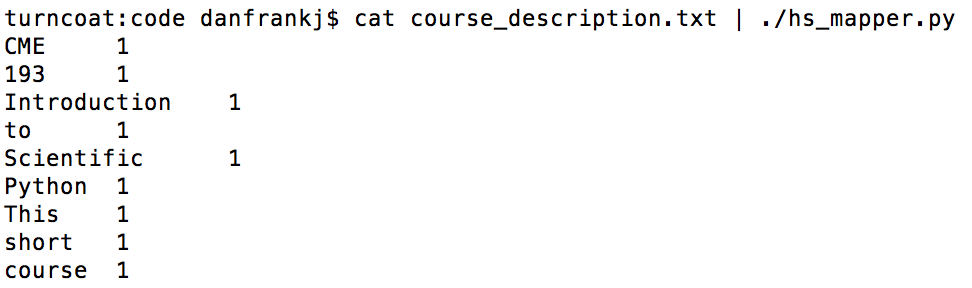
\includegraphics[width=.95\textwidth]{images/local1.png}
\end{figure}
\end{frame}

\begin{frame}
\frametitle{Hadoop Streaming: Testing}
\begin{figure}[h]
\centering
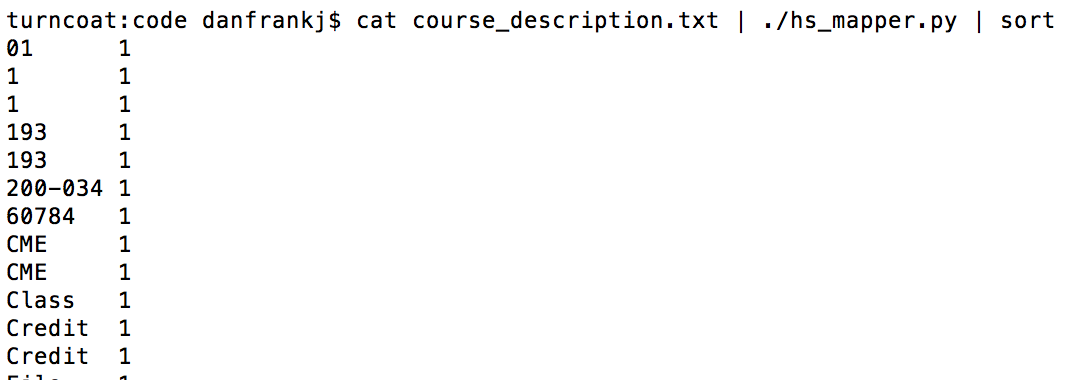
\includegraphics[width=.95\textwidth]{images/local2.png}
\end{figure}
\end{frame}

\begin{frame}
\frametitle{Hadoop Streaming: Testing}
\begin{figure}[h]
\centering
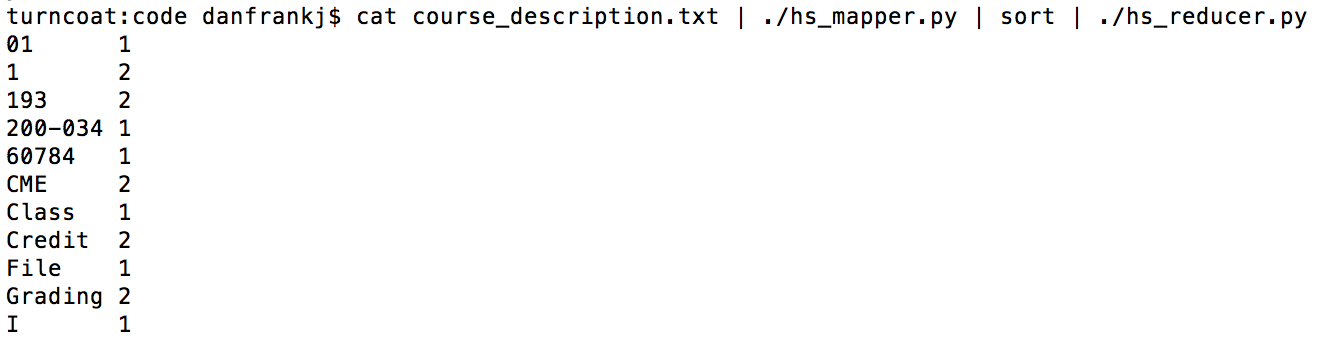
\includegraphics[width=.95\textwidth]{images/local3.png}
\end{figure}
\end{frame}

\begin{frame}
\frametitle{Hadoop Streaming: On Your Cluster}
\begin{enumerate}
\item copy local data to HDFS
\item launch job
\item monitor job status
\item collect output
\end{enumerate}
\end{frame}


\begin{frame}
\frametitle{Hadoop Streaming: Copying local data}
First we need to copy local data into HDFS so that our jobs can find it
\codeblock{code/hadoop_copy.sh}
\end{frame}

\begin{frame}
\frametitle{Hadoop Streaming: Launching the Job}
Once our cluster is configured we can launch the job with...
\codeblock{code/hadoop_wordcount.sh}
\end{frame}	

\begin{frame}
\frametitle{Hadoop Streaming: Monitoring Job Status}
\textcolor{blue}{\href{}{http://localhost:50030/}}
\texttt{http://localhost:50030/}
\end{frame}

\begin{frame}
\frametitle{Hadoop Streaming: Collecting Output}
\codeblock{code/hadoop_output.sh}

\end{frame}


\end{document}


